\documentclass{article} % For LaTeX2e
\usepackage{nips14submit_e,times}
\usepackage{amsmath}
\usepackage{amsthm}
\usepackage{amssymb}
\usepackage{mathtools}
\usepackage{hyperref}
\usepackage{url}
\usepackage{algorithm}
\usepackage[noend]{algpseudocode}
%\documentstyle[nips14submit_09,times,art10]{article} % For LaTeX 2.09

\usepackage{graphicx}
\usepackage{caption}
\usepackage{subcaption}

\def\eQb#1\eQe{\begin{eqnarray*}#1\end{eqnarray*}}
\def\eQnb#1\eQne{\begin{eqnarray}#1\end{eqnarray}}
\providecommand{\e}[1]{\ensuremath{\times 10^{#1}}}
\providecommand{\pb}[0]{\pagebreak}
\DeclarePairedDelimiter\ceil{\lceil}{\rceil}
\DeclarePairedDelimiter\floor{\lfloor}{\rfloor}

\newcommand{\E}{\mathrm{E}}
\newcommand{\Var}{\mathrm{Var}}
\newcommand{\Cov}{\mathrm{Cov}}

\def\Qb#1\Qe{\begin{question}#1\end{question}}
\def\Sb#1\Se{\begin{solution}#1\end{solution}}

\newenvironment{claim}[1]{\par\noindent\underline{Claim:}\space#1}{}
\newtheoremstyle{quest}{\topsep}{\topsep}{}{}{\bfseries}{}{ }{\thmname{#1}\thmnote{ #3}.}
\theoremstyle{quest}
\newtheorem*{definition}{Definition}
\newtheorem*{theorem}{Theorem}
\newtheorem*{lemma}{Lemma}
\newtheorem*{question}{Question}
\newtheorem*{preposition}{Preposition}
\newtheorem*{exercise}{Exercise}
\newtheorem*{challengeproblem}{Challenge Problem}
\newtheorem*{solution}{Solution}
\newtheorem*{remark}{Remark}
\usepackage{verbatimbox}
\usepackage{listings}
\usepackage{mathrsfs}
\title{ProbLimI: \\
Pset I}


\author{
Youngduck Choi \\
CIMS \\
New York University\\
\texttt{yc1104@nyu.edu} \\
}


% The \author macro works with any number of authors. There are two commands
% used to separate the names and addresses of multiple authors: \And and \AND.
%
% Using \And between authors leaves it to \LaTeX{} to determine where to break
% the lines. Using \AND forces a linebreak at that point. So, if \LaTeX{}
% puts 3 of 4 authors names on the first line, and the last on the second
% line, try using \AND instead of \And before the third author name.

\newcommand{\fix}{\marginpar{FIX}}
\newcommand{\new}{\marginpar{NEW}}

\nipsfinalcopy % Uncomment for camera-ready version

\begin{document}


\maketitle

\begin{abstract}
This work contains solutions to the exercises of the problem set I.
\end{abstract}

\bigskip

\begin{question}[1]
\hfill
\begin{figure}[h!]
  \centering
    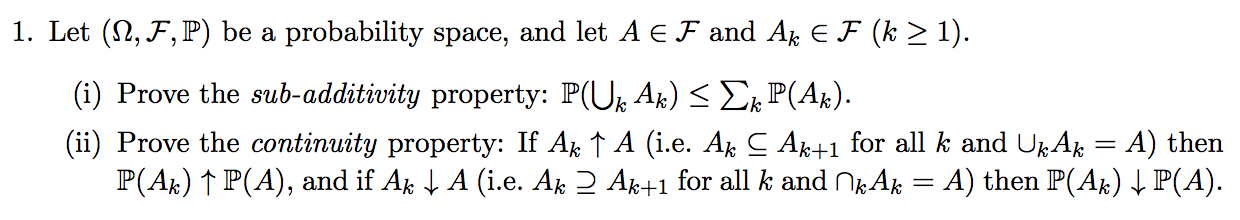
\includegraphics[width=0.7\textwidth]{problim-e1-p1.png}
\end{figure}
\end{question}
\begin{solution} \hfill \\

\end{solution}

\newpage

\begin{question}[2]
\hfill
\begin{figure}[h!]
  \centering
    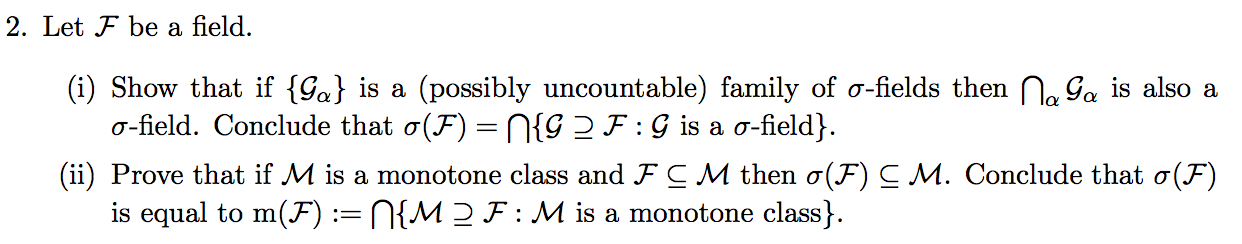
\includegraphics[width=0.7\textwidth]{problim-e1-p2.png}
\end{figure}
\end{question}
\begin{solution} \hfill \\
\textbf{(i)}
As $\emptyset$ and $\Omega$ are in $\mathscr{G}_{\alpha}$ for all $\alpha$,
by the $\sigma -$field property of each $\mathscr{G}_{\alpha}$, 
it follows that $\emptyset, \Omega \in \bigcap_{\alpha}
\mathscr{G}_{\alpha}$. Now, it suffices to show
that
\eQb
A \in \bigcap_{\alpha} \mathscr{G}_{\alpha} &\implies& 
A^c \in \mathscr{G}_{\alpha}, 
\\
\{ A_n\} \subset \bigcap_{\alpha} \mathscr{G}_{\alpha}  &\implies& 
\bigcap_n A_n \in \bigcap_{\alpha} \mathscr{G}_{\alpha}.
\eQe
If $A \in \bigcap_{\alpha} \mathscr{G}_{\alpha}$ then, $A \in \mathscr{G}_{\alpha}$
for all $\alpha$, and by the $\sigma -$field assumption on each $\mathscr{G}_{\alpha}$,
it follows that $A^c \in \mathscr{G}_{\alpha}$ for all $\alpha$, so $A^c \in
\bigcap_{\alpha} \mathscr{G}_{\alpha}$. \\ 

\smallskip

If $\{A_n \} \subset \bigcap_{\alpha} \mathscr{G}_{\alpha}$, then $\{ A_n \} \subset
\mathscr{G}_{\alpha}$ for all $\alpha$, and by the $\sigma -$ field assumption on
each $\mathscr{G}_{\alpha}$, it follows that $\bigcap_n A_n \in \mathscr{G}_{\alpha}$
for all $\alpha$, so $\bigcap_n A_n \in \bigcap_{\alpha} \mathscr{G}_{\alpha}$. 

\smallskip

Now, recall that $\sigma(\mathscr{F})$ is defined to be the smallest $\sigma$-field
containing $\mathscr{F}$. Consider the family of $\sigma$-field that contains 
$\mathscr{F}$, and denote it by $\{ \mathscr{G}_\alpha \}$.  
The above result shows that $\bigcap_{\alpha} 
\mathscr{G}_{\alpha}$ is a $\sigma$-field, and it is trivial that it contains
$\mathscr{F}$. Obviously, for any $\alpha$, $
\bigcap_{\alpha} \mathscr{G}_\alpha \subset \mathscr{G}_{\alpha}$, 
which tells us that any $\sigma$-algebra
containing $\mathscr{F}$ contains $\mathscr{G}_{\alpha}$, so it follows that
$\bigcap_{\alpha} \mathscr{G}_{\alpha}$ is the smallest $\sigma$-algebra containing
$\mathscr{F}$ and notationally we have 
\eQb
\sigma(\mathscr{F}) &=& \{ \mathscr{F} \subset \mathscr{G} : \mathscr{G} \> 
\text{ is a } \sigma-\text{field} \},
\eQe 
as required. \hfill $\qed$ 

\textbf{(ii)}   

\end{solution}

\newpage

\begin{question}[3]
\hfill
\begin{figure}[h!]
  \centering
    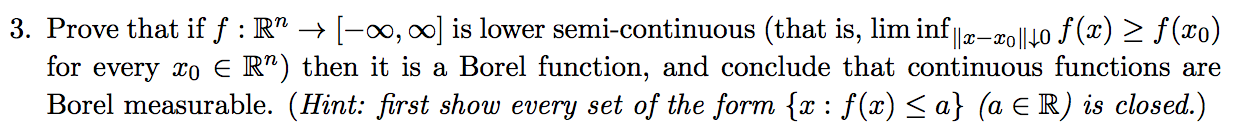
\includegraphics[width=0.7\textwidth]{problim-e1-p3.png}
\end{figure}
\end{question}
\begin{solution} \hfill \\

\end{solution}

\newpage 

\begin{question}[4]
\hfill
\begin{figure}[h!]
  \centering
    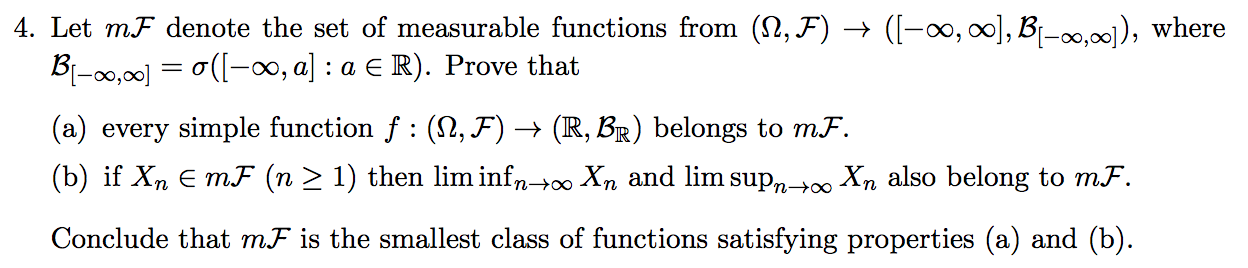
\includegraphics[width=0.7\textwidth]{problim-e1-p4.png}
\end{figure}
\end{question}
\begin{solution} \hfill \\

\end{solution}
\newpage

\end{document}
